\section{3D Transform}
A general matrix representation can be derived starting from all the transformations found so far :
\begin{figure}[H]
\centering
  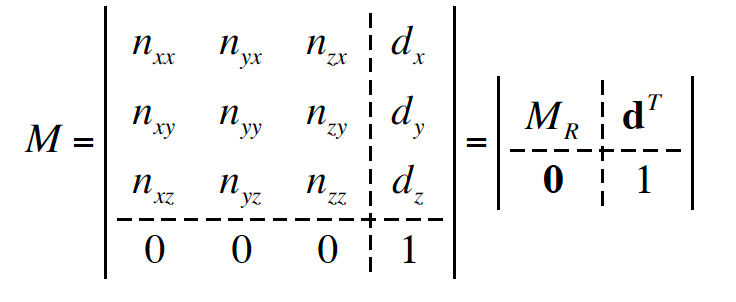
\includegraphics[width=.4\linewidth]{generalmatrix}
\end{figure}
\begin{itemize}
\item \textbf{Mr} : sub-matrix representing \textbf{rotation,scaling \& shear}
\item \textbf{dt} : translation
\item \textbf{1}  : to ensure that the w coordinate remains \textbf{unchanged}
\end{itemize}
The columns of $M_R$ represent \textbf{directions \& sizes} of the new axes in the old reference system\\
\textbf{Rotations} maintain the size of the axis constant but change their direction.\\
\textbf{Scalings} maintain the direction of the axis constant , changing the size.\\

\begin{figure}[H]
\centering
  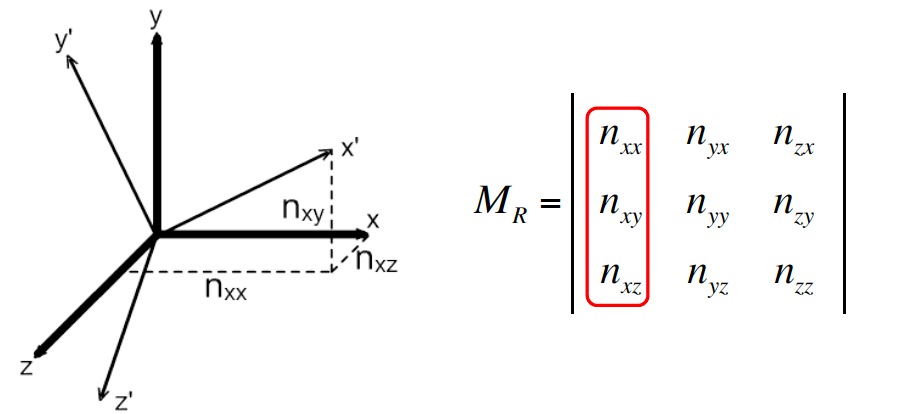
\includegraphics[width=.4\linewidth]{newaxis}
\end{figure}
Vector $d^t$ represents the position of the origin of the new coordinate system in the old one
\begin{figure}[H]
\centering
  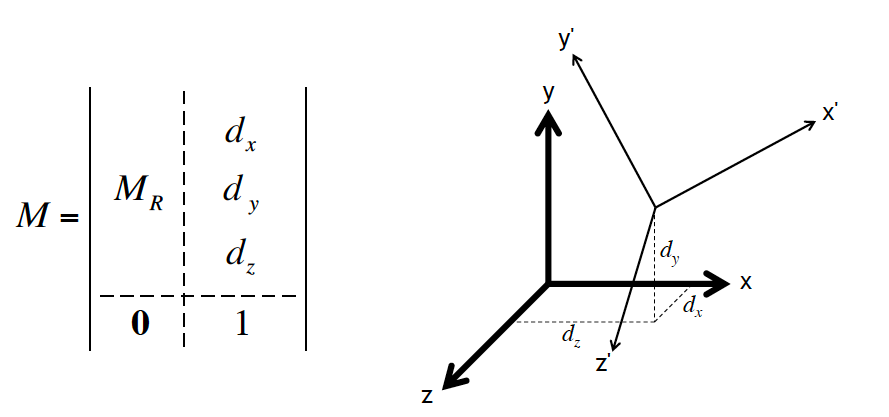
\includegraphics[width=.4\linewidth]{neworigin}
\end{figure}


\subsection{Inversion of transformations}
To return an object to its \textbf{origina} state transformation can be reversed. \textbf{Matrix inversion} can be applied when using the matrices representation of transformations.
$$ p'=(x',y',z',1) \to p=(x,y,z,1)$$
$$ p =M^{-1}p$$
Matrix $M^{-1}$ is \textbf{invertible} if its submatrix $M_R$ is invertible.
Generally $M^{-1}$ is always invertible except when dealing axis degeneration ( zero factor scaling for example).\\
Another method of inverting transformations is by using a reverse matrix : 
\begin{figure}[H]
\begin{minipage}{.5\textwidth}
 \centering
  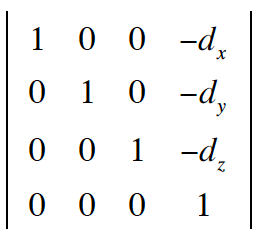
\includegraphics[width=.6\linewidth]{reversetr}
  \caption{Translation}
\end{minipage}%
	\begin{minipage}{.5\textwidth}
  \centering
  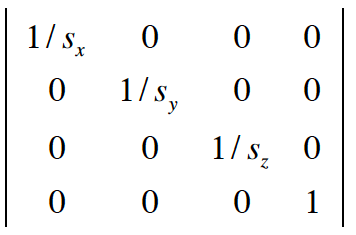
\includegraphics[width=.7\linewidth]{reversesc}
  \caption{Scaling}
\end{minipage}%
\end{figure}
\begin{figure}[H]
\begin{minipage}{.325\textwidth}
 \centering
  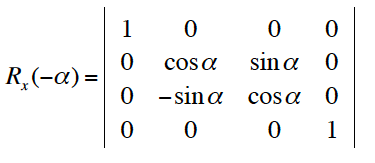
\includegraphics[width=.9\linewidth]{reversero3}
\end{minipage}%
	\begin{minipage}{.325\textwidth}
  \centering
  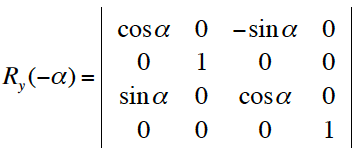
\includegraphics[width=.9\linewidth]{reversero2}
\end{minipage}%
\begin{minipage}{.35\textwidth}
  \centering
  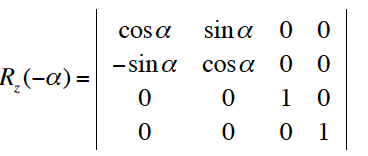
\includegraphics[width=.9\linewidth]{reversero1}
\end{minipage}%
\caption{Reverse rotation}
\end{figure}
\newpage
\subsection{Composition}
During the creation of scene an object is subject to \textbf{several} transformations. Applying a \textbf{sequence of transformations} is called \textbf{composition}.
An example is the movement of a cube , sides parallel to x,y,z axis and with center in the origin.\\
- Translation of center to position $p_x,p_y,p_z$\\
- Rotation of angle $\alpha$ around y\\
\begin{figure}[H]
  \centering
  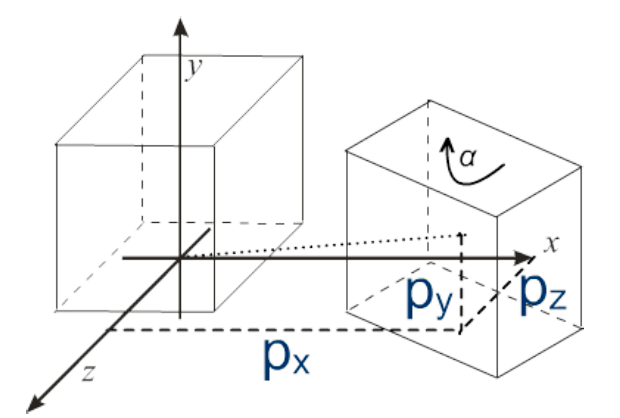
\includegraphics[width=.4\linewidth]{composition}
\end{figure}
\begin{itemize}
\item \textbf{Rotation} around y of $\alpha \to p'=R_y(\alpha) \cdot p$\\
$	
R_y(\alpha)= \begin{bmatrix}
       cos\alpha & 0 & sin\alpha & 0        \\[0.1em]
       0 & 1 & 0 & 0		    \\[0.1em]
       -sin\alpha & 0 & cos\alpha & 0							\\[0.1em]
       0 & 0 & 0 & 1
     \end{bmatrix} 
$ 
\item \textbf{Translation} in position $p''=T(p_x,p_y,p_z) \cdot p'$\\
$	
T(p_x,p_y,p_z)= \begin{bmatrix}
       1 & 0 & 0 & p_x        \\[0.1em]
       0 & 1 & 0 & p_y	    \\[0.1em]
       0 & 0 & 1 & p_z							\\[0.1em]
       0 & 0 & 0 & 1
     \end{bmatrix} 
$
\end{itemize}
\[
\boxed{p''= T(p_x,p_y,p_z) \cdot R_y(\alpha) \cdot p}
\]
Matrices appear in \textbf{reverse} order wrt to the transformations they represent.
\subsubsection{Properties of composition of transformations}
Matrix-Matrix and Matrix-Vector products are \textbf{associative}:
$$ A \cdot (B \cdot C) = (A \cdot B) \cdot C$$
$$ A \cdot (B \cdot p) = (A \cdot B) \cdot p$$
Using the associative property we can obtain a \textbf{single matrix} corresponding to the product of \textbf{all the transformations}.\\
This is useful because usually the multiplication is done for many points ($ 10^4 \sim 10^6$ , so having one matrix that sums up all transformation \textbf{improves performances}.\\
\begin{figure}[H]
  \centering
  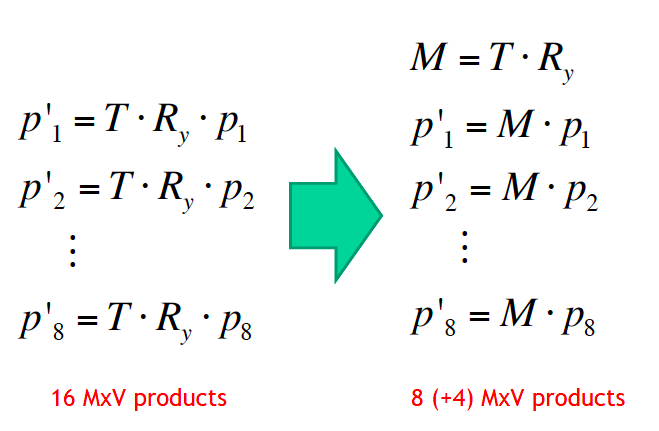
\includegraphics[width=.4\linewidth]{comp-prop}
\end{figure}
As in the figure instead of having 16 matrix-vector products we only have 12 ( 4 are to create the matrix M ).\\
\textbf{Inversion} can be handled by considering : $$ (A \cdot B)^{-1} = B^{-1} \cdot A^{-1}$$
Example : $M= R_y(\ang{30}) \cdot T(1,2,3) \to M^{-1}= T(1,2,3)^{-1} \cdot R_y(\ang{30})^{-1}$
Matrix products are \textbf{not commutative} : the order of the transformations is important , and transformations cannot be swapped without obtaining a \textbf{different } result.
\newpage
\subsection{Transformations around an arbitrary axis or center}
\begin{description}
\item[Case : Rotation]\hfill\\
Instead of rotating an object around the x,y or z axis we consider now a rotation of angle $\alpha$ around an arbitrary axis that passes through the origin. Depending on where the considered axis is it forms \textbf{two angles} with the the other axis.
\begin{figure}[H]
  \centering
  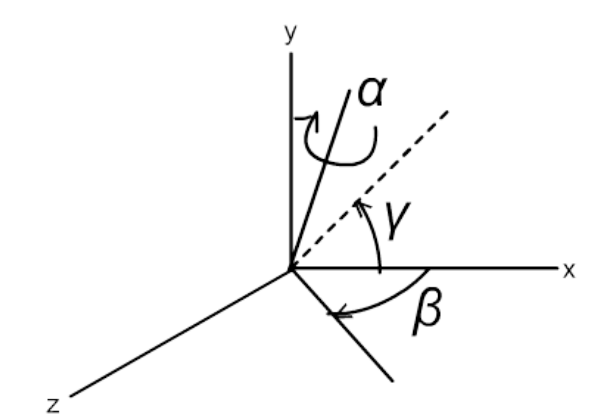
\includegraphics[width=.4\linewidth]{axis}
\end{figure}
In this case the two angles are $\gamma, \beta$ :\\
- $\gamma \to$ how much the axis rises on the xz plane\\
- $\beta \to$ how much it rises on the xy plane\\
The angles and planes chosen are arbitrary, other angles and planes can be used to describe the same transformations.
\begin{enumerate}
\item $R_y(-\beta)$\\
Considering a rotation of $-\beta$  along the y-axis ,the arbitrary axis now lies on the xy plane.
\item $R_z(-\gamma)$\\
Then considering a rotation of $-\gamma$ along the z-axis ,the arbitrary axis now corresponds to the x-axis.
\item $R_x(\alpha)$\\
As our chosen axis corresponds to the x-axis , the rotation of the object of angle $\alpha$ can be done around the x-axis.
\item $R_z(\gamma)$ and $R_y(\beta)$\\
To restore the original axis position.
\end{enumerate}
Final transformation composition :
\[
\boxed{p'=R_y(\beta)R_z(\gamma)R_x(\alpha)R_Z(-\gamma)R_y(-\beta) \cdot p}
\]

If the axis does not pass through the \textbf{origin} , a \textbf{translation T} must be applied of a point known through which the axis passes:
\[
\boxed{p'=T(p_x,p_y,p_z)R_y(\beta)R_z(\gamma)R_x(\alpha)R_Z(-\gamma)R_y(-\beta)T(-p_x,-p_y,-p_z) \cdot p}
\]

Similar procedures can be applied to :
\begin{itemize}
\item \textbf{Scaling}
\item \textbf{Shear}
\end{itemize}
\end{description}



